\section{Enregister un capteur}\label{sec:enregistrer-un-capteur}

    \begin{figure}[H]
        \begin{center}
            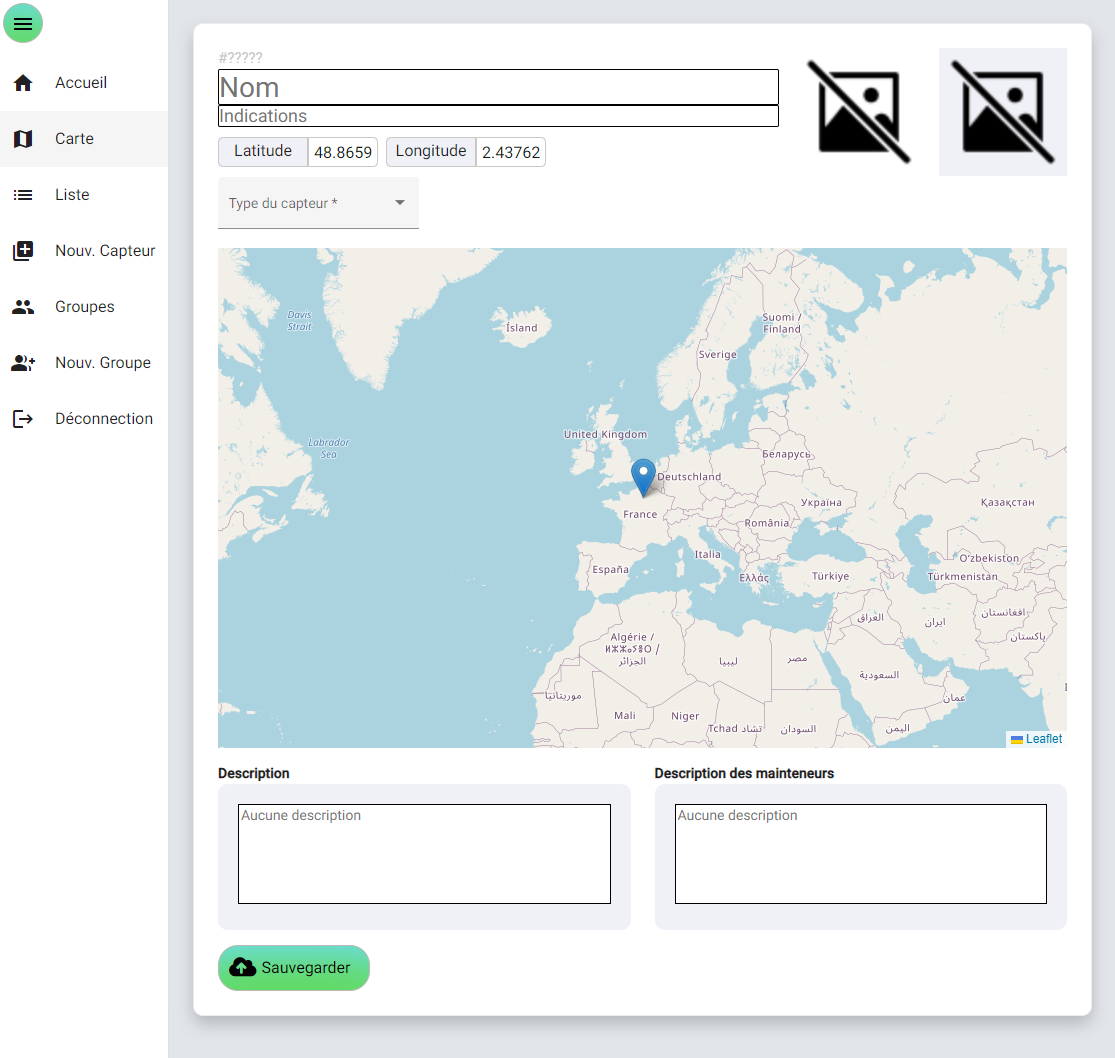
\includegraphics[width=12cm]{resources/create_sensor}
        \end{center}
        \caption{Page de création de capteur}\label{fig:create-sensor}
    \end{figure}

    Pour créer un capteur, vous devez être connecté.
    Après votre connexion vous devrez vous rendre sur ``Nouv. Capteur'' dans le menu.
    Une fois ceci, fais, il vous faut remplir le nom, les indications, l'image, le type du capteur,
    sélectionner l'aide de la carte l'emplacement du cpateur.
    Attention, vous ne pourrez plus changer la position de votre capteur,
    il faudra en recrée un si vous souhaiter le déplacer.
    Vous pouvez aussi ajouter une description à destination des visiteurs ou des mainteaneurs.

    Une fois les informations complété, vous pourrez sauvegarder le capteur et serez directement rediriger vers la page nouvellement créée.

    \clearpage